\section{Symbolic Aggregate approXimation (SAX)}
The last approach for the time-series similarity problem we are reviewing in this writing is the current state of the art time-series representation and dimentionality reduction method called Symbolic Aggregate approXimation (SAX) which transforms original time-series data into symbolic strings. This method, proposed by Lin et al \cite{citeulike:2821475}, turns out to be not only extremely simple and computationally cheap, but also fast and precise in the range-query processing. Moreover, the use of the symbolic representation opens door to the existing wealth of data-structures and string-manipulation algorithms in computer science such as hashing, suffix trees, regular expression pattern matching, etc.

SAX transforms a time-series $X$ of length $n$ into the string of arbitrary length $\omega$ where typically $\omega << n$, using an alphabet $A$ of size $ a \geq 2$. The SAX algorithm consis of two steps: at the first step it transforms the original time-series into PAA representation and this intermediate representation than converted into the string during the second step. Use of the PAA at the first step brings an advantage of simple and efficient dimensionality reduction while providing the important lower bounding property. Second step, actual conversion of PAA coefficients into letters also computationally efficient and the lower bounding of symbolic distance was proven by Lin et al.

Discretization of the PAA representation of the time-series into SAX implemented in a way which produces symbols corresponding to the time-series features with equal probability. The rigorous analysis of the time-series datasets available for authors shows that normalized by the zero mean and unit of energy time-series follow the Normal distribution law. By using the Gaussian distribution properties \cite{citeulike:167581} it's easy to pick $a$ equal-sized areas under the Normal curve. The points of the cut lines slicing the the under-the-Gaussian-curve area called ``breakpoints''.
\begin{figure}[tbp]
   \centering
   \includegraphics[height=45mm]{sax_intro.eps}
   \caption{The illustration of the SAX approach taken from \cite{citeulike:2821475} depicts two pre-determined breakpoints for the three-symbols alphabet and the conversion of the time-series of length $n=128$ into PAA representation first and following mapping of the PAA coefficients into SAX symbols with $w=8$ and $a=3$ resulting in the string \textbf{baabccbc}.}
   \label{fig:sax_intro}
\end{figure}

Extending Euclidean \ref{eq:euclidean_distance} and PAA \ref{eq:paa_distnace} distances, the function returning the minimal distance between two string representations of original time series $\hat{Q}$ and $\hat{C}$ defined as
\begin{equation}
MINDIST(\hat{Q},\hat{C}) \equiv \sqrt{ \frac{n}{w} } \sqrt{ \sum_{i=1}^{w} ( dist( \hat{q}_{i}, \hat{c}_{i} ) )^{2}}
\label{eq:sax_mindist}
\end{equation} 
where the $dist$ function is implemented by using the lookup table for the particular set of the breakpoints as shown in table \ref{tbl:sax_lookup} where the singular value for each cell $(r,c)$ is computed as 
\begin{equation}
cell_{(r,c)} = 
\begin{cases} 
0, \text{ if }\left| r-c \right| \leq 1 \\
\beta_{\max(r,c) - 1} - \beta_{\min(r,c) - 1}, \text{ otherwise}
\end{cases}
\label{eq:cell}
\end{equation}
\begin{table}
\begin{tabularx}{400pt}{X X X X X}
\hline
   & a   & b    & c    & d    \\
\hline
a & 0    & 0    & 0.67 & 1.34 \\
b & 0    & 0    & 0    & 0.67 \\
c & 0.67 & 0    & 0    & 0    \\
d & 1.34 & 0.67 & 0    & 0    \\
\hline
\end{tabularx}
\caption{A lookup table used by the MINDIST function for the $a=4$}
\label{tbl:sax_lookup}
\end{table}
\begin{figure}[tbp]
   \centering
   \includegraphics[height=47mm]{sax_distance.eps}
   \caption{The visual representation of the two time-series $Q$ and $C$ and three distances between their representation: Euclidean distance between raw time-series (A), the distance defined for PAA coefficients (B) and the distance between two SAX representations (C).}
   \label{fig:sax_distance}
\end{figure}


As shown by Li et al, the introduced SAX distance measure lower-bounds the PAA distance, i.e.
\begin{equation}
\sum_{i=1}^{n} (q_{i} - c_{i})^{2} \geq n(\bar{Q} - \bar{C})^{2} \geq n(dist(\hat{Q},\hat{C}))^2
\label{eq:sax_bounding}
\end{equation}
